\documentclass[tikz, border=2pt]{standalone}

\usepackage[utf8]{inputenc}
\usepackage{tikz}
\usetikzlibrary{mindmap}
\renewcommand{\familydefault}{\sfdefault}



\definecolor{julia_blue}{rgb}{0.251, 0.388, 0.847}
\definecolor{julia_purple}{rgb}{0.584, 0.345, 0.698}
\definecolor{julia_green}{rgb}{0.22, 0.596, 0.133}
\definecolor{julia_red}{rgb}{0.796, 0.235, 0.2}

\begin{document}

\begin{tikzpicture}[mindmap, grow cyclic, concept color=black,
        level 1/.append style={level distance=5cm,sibling angle=120},
        level 2/.append style={level distance=3cm,sibling angle=60},
        level 3/.append style={level distance=2cm,sibling angle=37}]

\node [concept, fill=white] (AIBECS) {}
child [concept color=julia_purple!40, sibling angle=170] { node [concept] {Observational Data}
    child [concept color=julia_red!40!white] { node [concept] {GEO-\\TRACES}
        child { node [concept] {Iron}}
        child { node [concept] {Cobalt}}
        child { node [concept] {Zink}}
    }
    child [concept color=julia_red!40!white] { node [concept] {BCO-DMO}
        child { node [concept] {PON}}
        child { node [concept] {POP}}
        child { node [concept] {POC}}
    }
    child [concept color=julia_green!40] { node [concept] {World Ocean Atlas}
        child { node [concept] {O\textsubscript{2}}}
        child { node [concept] {PO\textsubscript{4}}}
        child { node [concept] {NO\textsubscript{3}}}
        child { node [concept] {Si(OH)\textsubscript{4}}}
    }
}
child [concept color=julia_purple!40] { node [concept] {Ocean Circulations}
    child [concept color=julia_green!40,sibling angle=28] { node [concept] {OCIM0}}
    child [concept color=julia_green!40,sibling angle=28] { node [concept] {OCIM1}}
    child [concept color=julia_green!40,sibling angle=28] { node [concept] {Archer et al.}}
    child [concept color=julia_green!40,sibling angle=28] { node [concept] {ShoeBox}}
    child [concept color= julia_blue!40,sibling angle=28] { node [concept] {OCCA}}
    child [concept color= julia_blue!40,sibling angle=28] { node [concept] {OCIM2}}
    child [concept color= julia_blue!40,sibling angle=28] { node [concept] {POP}}
    child [concept color=  julia_red!40,sibling angle=28] { node [concept] {MPAS-O}}
    child [concept color=  julia_red!40,sibling angle=28] { node [concept] {ACCESS}}
    child [concept color=  julia_red!40,sibling angle=28] { node [concept] {MITgcm}}
    child [concept color=  julia_red!40,sibling angle=28] { node [concept] {CYCL-\\OCIM}}
}
child [concept color=julia_purple!40, sibling angle=-100] { node [concept] {Optimization}
    child [concept color=julia_green!40] { node [concept] {Optim}}
    child [concept color=julia_green!40] { node [concept] {F1Method}}
}
;


\node (foo) at (AIBECS) {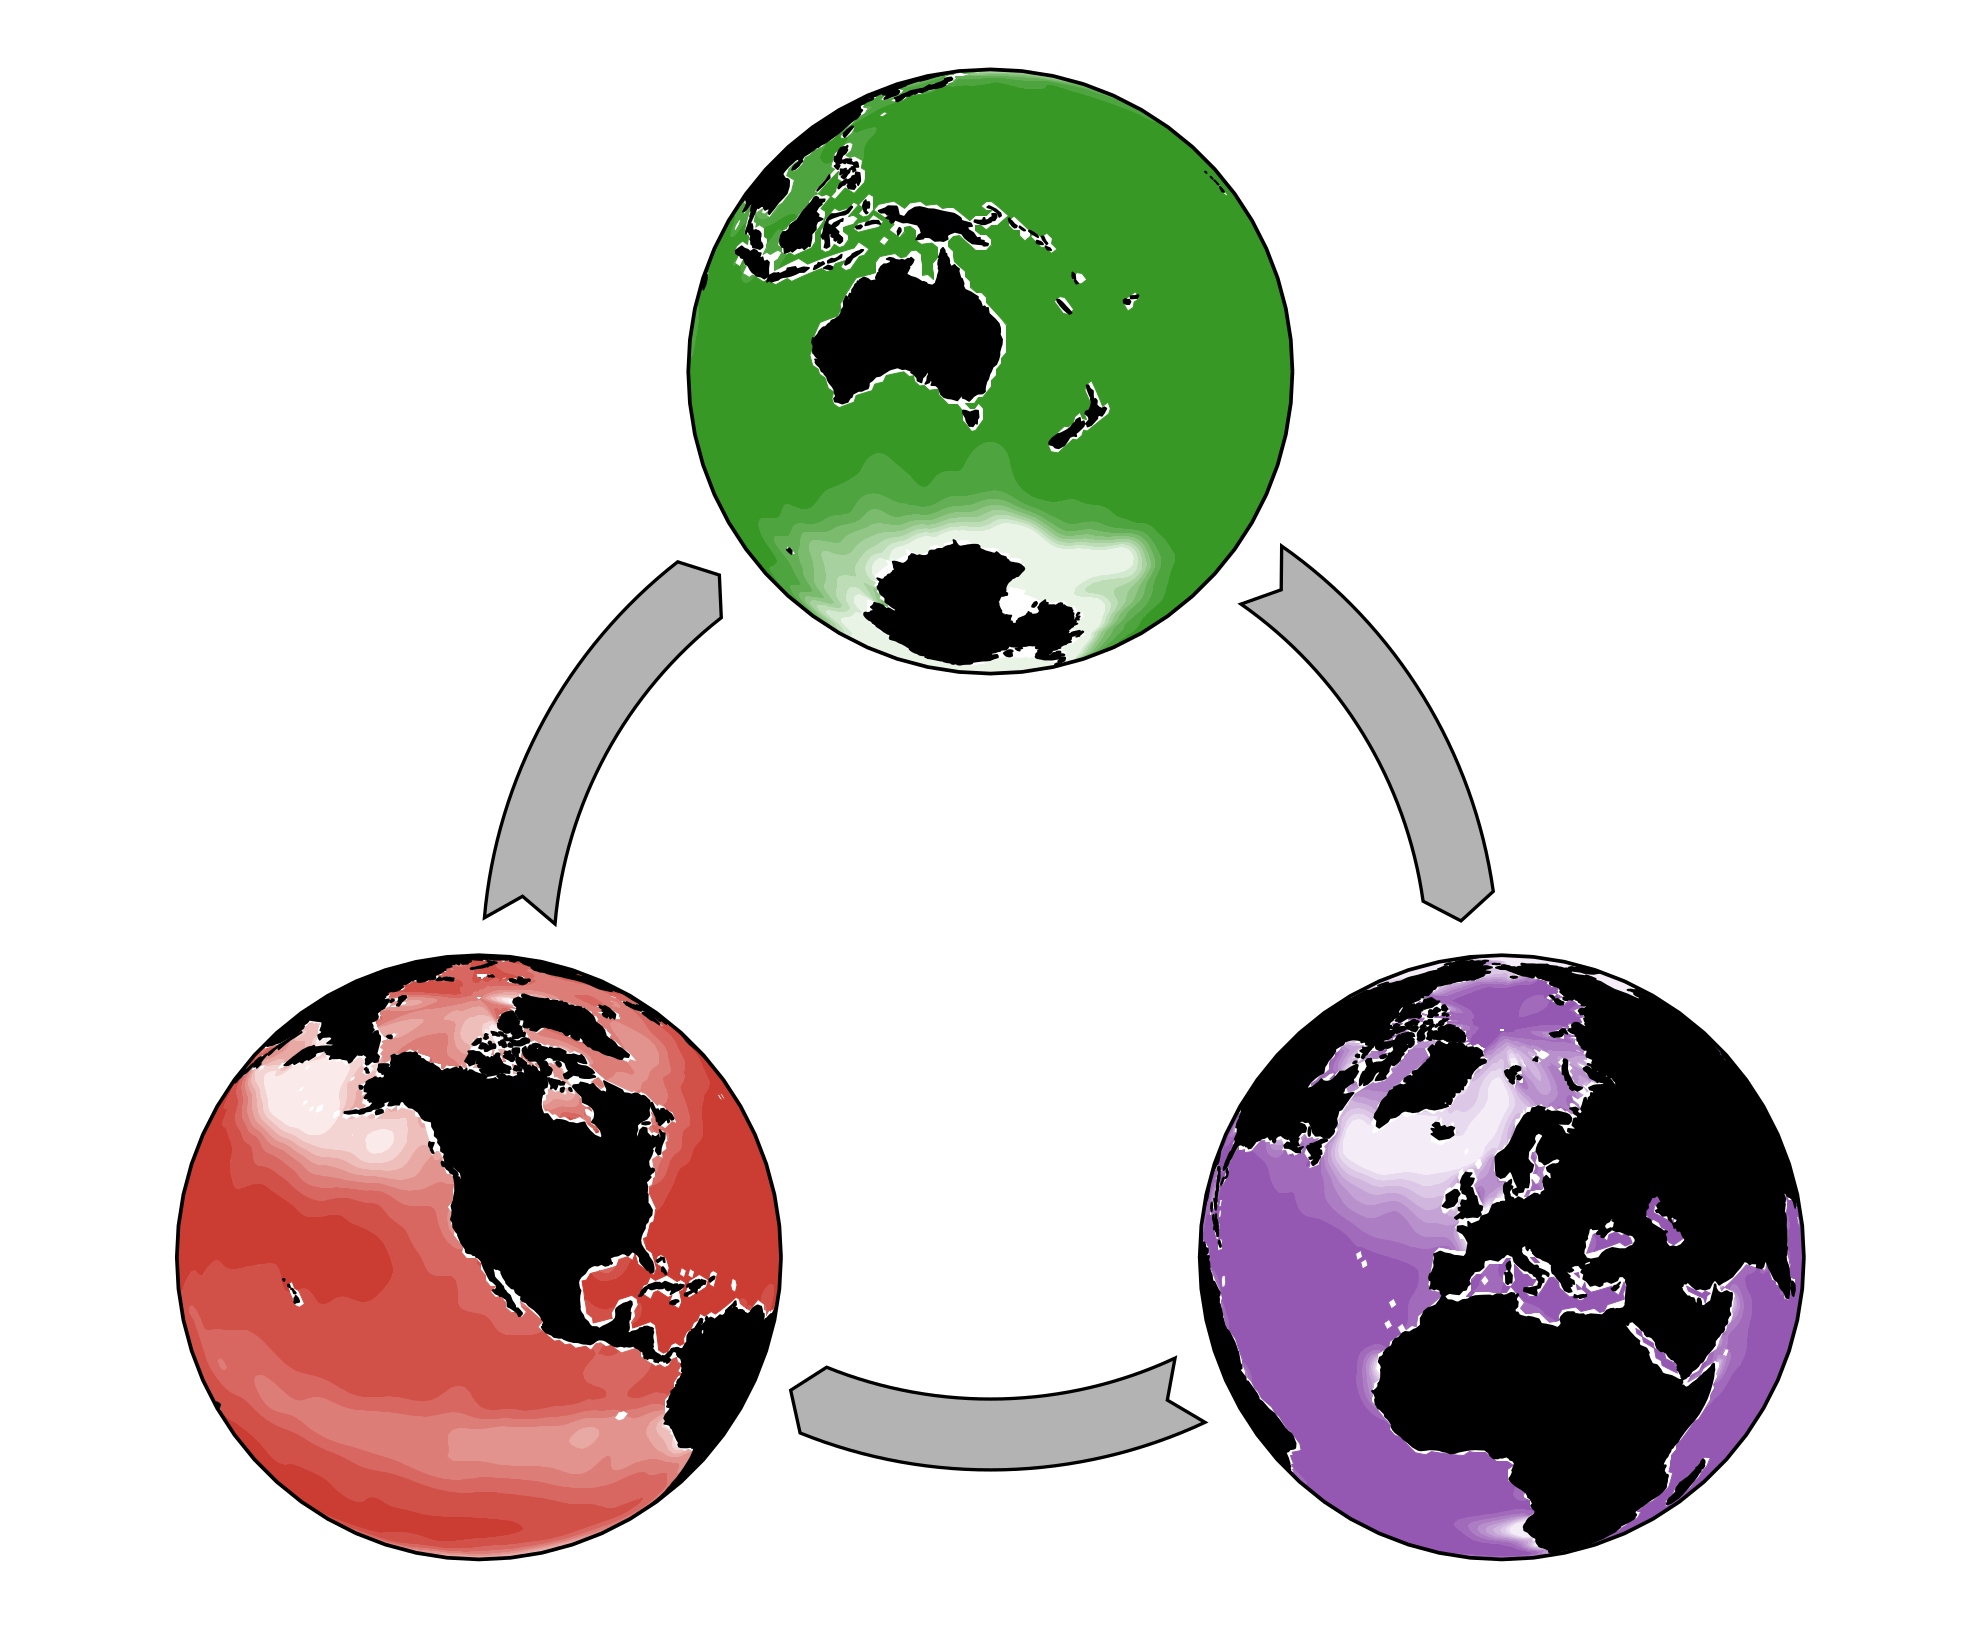
\includegraphics[width=3.4cm]{img/AIBECS_logo.png}\\\textbf{AIBECS.jl}};
\node (OG) at (5,-5) {
\includegraphics[trim=50 40 50 0,clip,width=3cm]{img/OceanGrids_logo.png}\\\textbf{OceanGrids.jl}};
\node (WOAT) at (-7,-7.3) {
\includegraphics[width=4cm]{img/WOAT_logo.png}\\\textbf{WorldOceanAtlasTools.jl}};
\node (F1) at (2.5,-7.3) {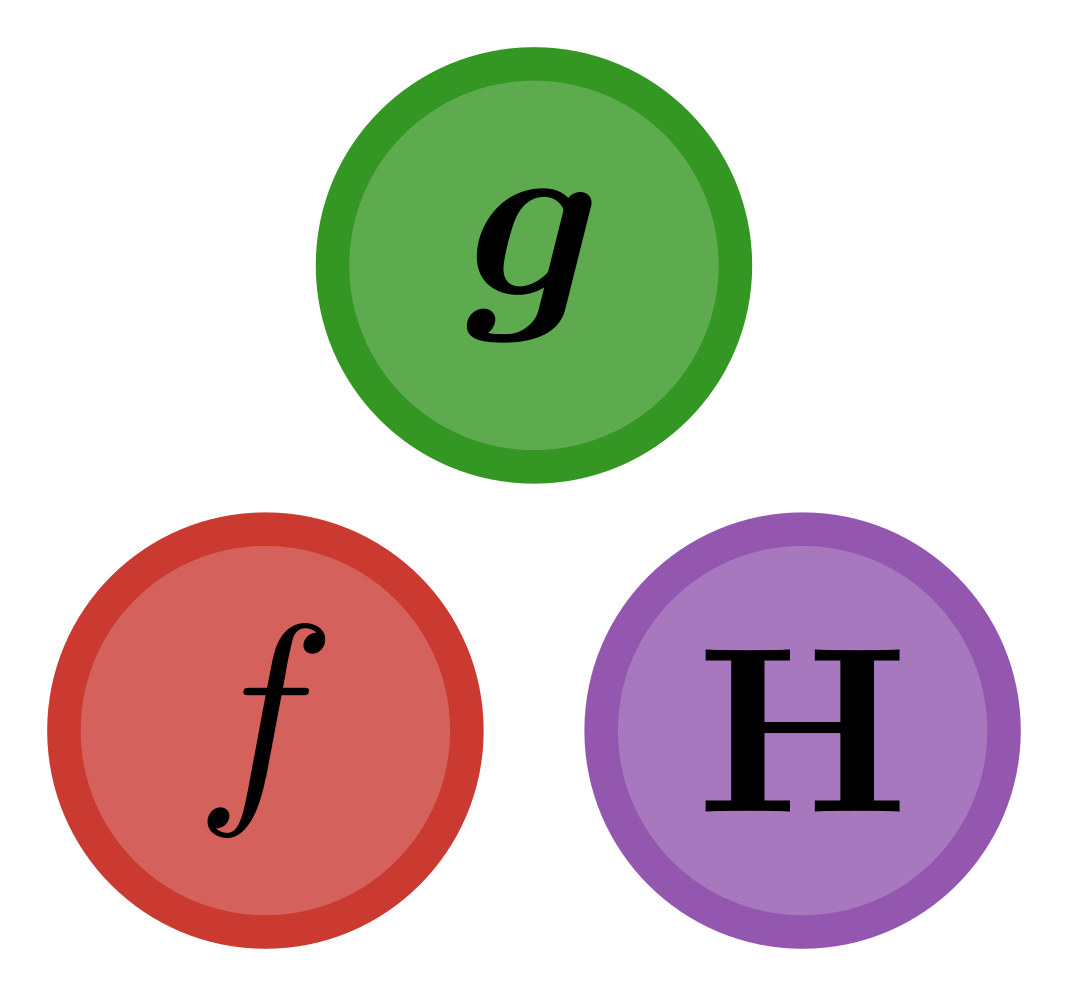
\includegraphics[width=1.8cm]{img/F1_logo.png}\\\textbf{F1Method.jl}};
\node [text width=7cm] (tit) at (-2,3) {\huge \bf AIBECS.jl ecosystem};

\end{tikzpicture}

\end{document}
